\chapter{Les modules d'extensions Moodle}

Le côté modulaire de Moodle est aussi développé pour les enseignants que pour les programmeurs.
Presque toutes les fonctionnalités de Moodle sont configurées à l'aide de modules d'extensions.
Il y a des modules d'extensions pour changer l'apparence du site, pour gérer les compétences SCORM, pour exporter les données, pour changer le fonctionnement des questions, etc.
Chaque module d'extension est développée par un membre de la communauté et est approuvée par un comité Moodle.

\begin{figure}[h!]
  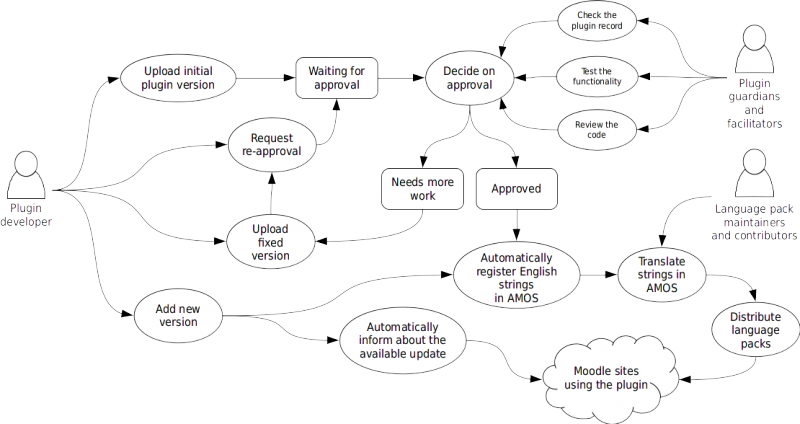
\includegraphics[scale=0.7]{images/plugin-contribution-workflow.png}
  \caption[Flux d'acception d'un module d'extension Moodle]{Flux d'acception d'un module d'extension Moodle, \href{https://docs.moodle.org/dev/Plugin_contribution}{\mbox{https://docs.moodle.org/dev/Plugin\_contribution}}}
\end{figure}

Pour ajouter des fonctionnalités à l'activité questionnaires, il y a trois types de module d'extensions à considérer: un rapport de questionnaire, un type de question et un comportement de question.

\section{Module d'extension rapport de questionnaire (\textit{Quiz report})}

Un rapport de questionnaire sert principalement à corriger les réponses des étudiants.
On peut aussi se servir de ce type de module d'extension pour afficher les réponses et les notes des étudiants pour un questionnaire sous forme de rapport.
On peut aussi s'en servir afin de modifier les champs disponibles dans la configuration de base d'un questionnaire.

Lors de l'analyse initiale du projet; il était prévu de se servir uniquement de ce type de module d'extension, car nous voulons uniquement modifier l'interface de correction.
Par contre, comme nous voulons ajouter une liste de mots clés à une question et que ce type de module d'extension permet de modifier seulement le questionnaire, un seul module d'extension de ce type ne sera pas suffisante.

\section{Module d'extension type de question (\textit{Question type})}

Chaque question est définie par un type de question (voir la liste à la section~1.1 de ce document).
Un nouveau type de question ajoute donc plus de choix à l'enseignant désirant créer un questionnaire.
Chaque type de question possède des champs personnalisés et change l'apparence de la question pour l'étudiant et l'enseignant.

On ne voulait pas modifier le module d'extension \og Type de question Composition \fg{} car les nouvelles fonctionnalités ne seront pas utiles pour tous les types de texte: un texte d'opinion pour un cours de philosophie, par exemple, n'aura aucune utilité d'une liste de mots-clés et de comparaison de textes.
La possibilité de créer un module d'extension qui ajoute un nouveau type de question qui étend les fonctionnalités du \og Type de question Composition \fg{} par héritage a été analysé, mais ce n'est pas possible avec Moodle.
Seule alternative restante: se baser sur le \og Type de question Composition \fg{} pour créer un tout nouveau module d'extension.
Ce nouveau module d'extension utilise les mêmes fonctionnalités que le \og Type de question Composition \fg{} en enlevant quelques fonctionnalités (remise de pièce jointe et écriture dans un WYSIWIG) et en ajoutant quelques autres (mots-clés et réponse de l'enseignant).

\section{Module d'extension comportement de question (\textit{Question behaviour})}

Un comportement de question permet de:
\begin{enumerate}
  \item Ajouter du code à la suite de la question, par exemple un bouton \og Vérifier \fg{} ou une zone de texte commentaire;
  
  \item Modifier la méthode de correction, par exemple une correction manuelle, une correction automatique instantanée quand l'étudiant répond ou une correction automatique lorsque le test est terminé;
  
  \item Modifier l'affichage des questions, par exemple afficher une question supplémentaire si l'étudiant a plusieurs fautes ou donner des indices à l'étudiant occasionnant une perte de points.
\end{enumerate}

Comme nous désirons une correction manuelle, nous pouvons utiliser le comportement \og ManualGraded \fg{}.
De plus, comme il est possible de contrôler directement l'apparence de la réponse et de la question avec le module d'extension \og Question type \fg{}, il n'est pas nécessaire de créer un module d'extension \og Comportement de question \fg{} pour modifier l'apparence de la question.

\section{Choix des modules d'extensions à créer}

Un module d'extension type de question est obligatoire dans ce projet afin d'ajouter les champs mots-clés et réponse de l'enseignant.
Nous n'avons pas besoin des fonctionnalités qu'offre le module d'extension comportement de question.
Il reste à déterminer s'il faut utiliser un module d'extension rapport de questionnaire ou non.

En analysant le code du module d'extension de correction manuelle fournie de base avec Moodle (quiz\_grading) on découvre qu'elle fournit l'interface de correction, mais que la réponse de chaque étudiant est gérée par le type de question dans un affichage en lecture seulement.
Les fonctionnalités prévues peuvent donc se trouver autant dans le type de question que dans un rapport de questionnaire, la complexité du code est la même pour les deux cas.
Puisqu'il doit y avoir obligatoirement un module d'extension type de question et qu'une nouveau module d'extension rapport de questionnaire est facultative, il a été décidé de faire un seul module d'extension.
Le fait d'avoir un seul module d'extension facilite grandement l'installation pour d'autres administrateurs Moodle.